 \documentclass{report}
 
\usepackage[utf8]{inputenc} 
\usepackage[T1]{fontenc}      
\usepackage[top=2.0cm, bottom=3cm, left=3.0cm, right=3.0cm]{geometry}
\usepackage{graphicx}
\usepackage{wrapfig}
\usepackage{amsmath,esint }
\usepackage{amssymb}
\graphicspath{{figures/}{../figures}}

\newcommand*\dif{\mathop{}\!\mathrm{d}}
\newcommand*\diver{\mathop{}\!\mathrm{div}}
\newcommand*\grad{\mathop{}\!\mathrm{grad}}

\begin{document}

\section*{Alimentation à découpage}

La structure ci-dessous est une alimentation à découpage, alimentée par une source de tension continue de f.e.m $E=50$ V. On s'intéresse au fonctionnement périodique de période $T=50$ $\mu$s. La séquence de commande des interrupteurs est la suivante : pour $t\in[0,\alpha T[$, $K$ est fermé et $K'$ est ouvert ; pour $t\in[\alpha T, [$ $K$ est ouvert et $K'$ est fermé.

\begin{figure}[h!]
	\centering
		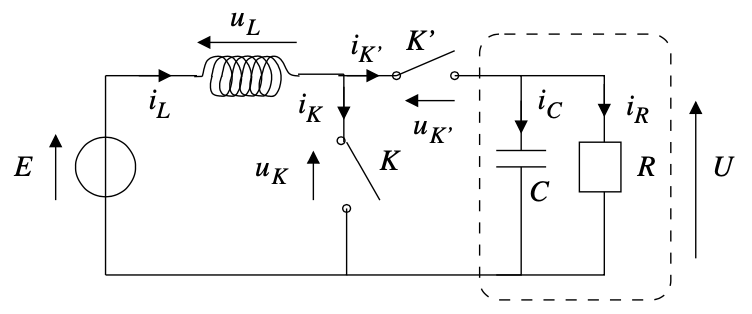
\includegraphics[scale=0.9]{circuit1.png}
\end{figure}	

On suppose dans un premier temps que l'association $R//C$ entourée en pointillée se comporte comme une source de tension idéale $U=E'$ et on se place dans l'hypothèse où le courant dans la bobine $L$ ne s'annule jamais. On note $I_m$ et $I_M$ les valeurs minimales et maximales de $i_L$.

\begin{itemize}

	\item[$\thicksim$] Calculer $\left\langle u_L \right\rangle$ de deux manières différentes et montrer que $U=E'=\frac{E}{1-\alpha}$.
	
	\item[$\thicksim$] On règle $\alpha$ à la valeur $\alpha=0,6$. On accepte pour l'utilisation voulue une ondulation $\Delta i=I_M-I_m$ au maximum de 0,3 A pour cette valeur de $\alpha$. Déterminer la valeur minimale $L_{min}$ de l'inductance $L$.
	
	\item[$\thicksim$] La puissance moyenne fournie par la source de tension est $P=150$ W pour $\alpha=0,6$. Pour $L=L_{min}$ déterminer $I_M$ et $I_m$.
	
	\item[$\thicksim$] La puissance moyenne fournie par la source de tension est $P=150$ W pour $\alpha=0,6$. Pour $L=L_{min}$ déterminer $I_M$ et $I_m$.
	
	\item[$\thicksim$] Tracer sur un chronogramme les caractéristiques courant-tension pour chaque interrupteur sur une période $T$ En déduire le fonctionnement, transistor ou diode, des interrupteurs. 
	
	\item[$\thicksim$] Quelle est la valeur moyenne $U_0$ de la tension $u_K$ aux bornes de l'interrupteur $K$ ? 

\end{itemize}

On se place toujours dans les conditions $P=150$ W pour $\alpha=0,6$. La tension $U$ aux bornes de l'association parralèle $R//C$ n'est pas constante : c'est une fonction périodique du temps qui présente une légère ondulation autour de sa valeur moyenne $E'$. On suppose que cela ne modifie pas les courants $i_L$, $i_K$ et $i_{K'}$.

\begin{itemize}

	\item[$\thicksim$] Déterminer littéralement les intensités moyennes $I_R$ et $I_C$ des courants dans la charge $R$ et dans le condensateur $C$ en fonction de $\alpha$, $R$ et $E$.
	
	\item[$\thicksim$] Déterminer numériquement les valeurs moyennes de $P_R$ et de $P_C$ des puissances dissipées dans $R$ et dans $C$.
	
\end{itemize}
	
\newpage

\section*{Alimentation par un hacheur en série}

On alimente un récepteur f.e.m. $E$ de résistance $R$ par un hacheur série selon le schéma ci-dessous. $E_{G}$ et $E$ sont positifs.

Les interrupteurs sont supposés parfaits, la période est $T$ et le rapport cyclique $\alpha$ : au cours de chaque période, l'interrupteur commandé est fermé pendant une durée $\alpha T$ puis ouvert pendant une durée $(1-\alpha)T$. On suppose que l'intensité $i$ qui traverse la bobine est quasiment constante.

\begin{figure}[h!]
	\centering
		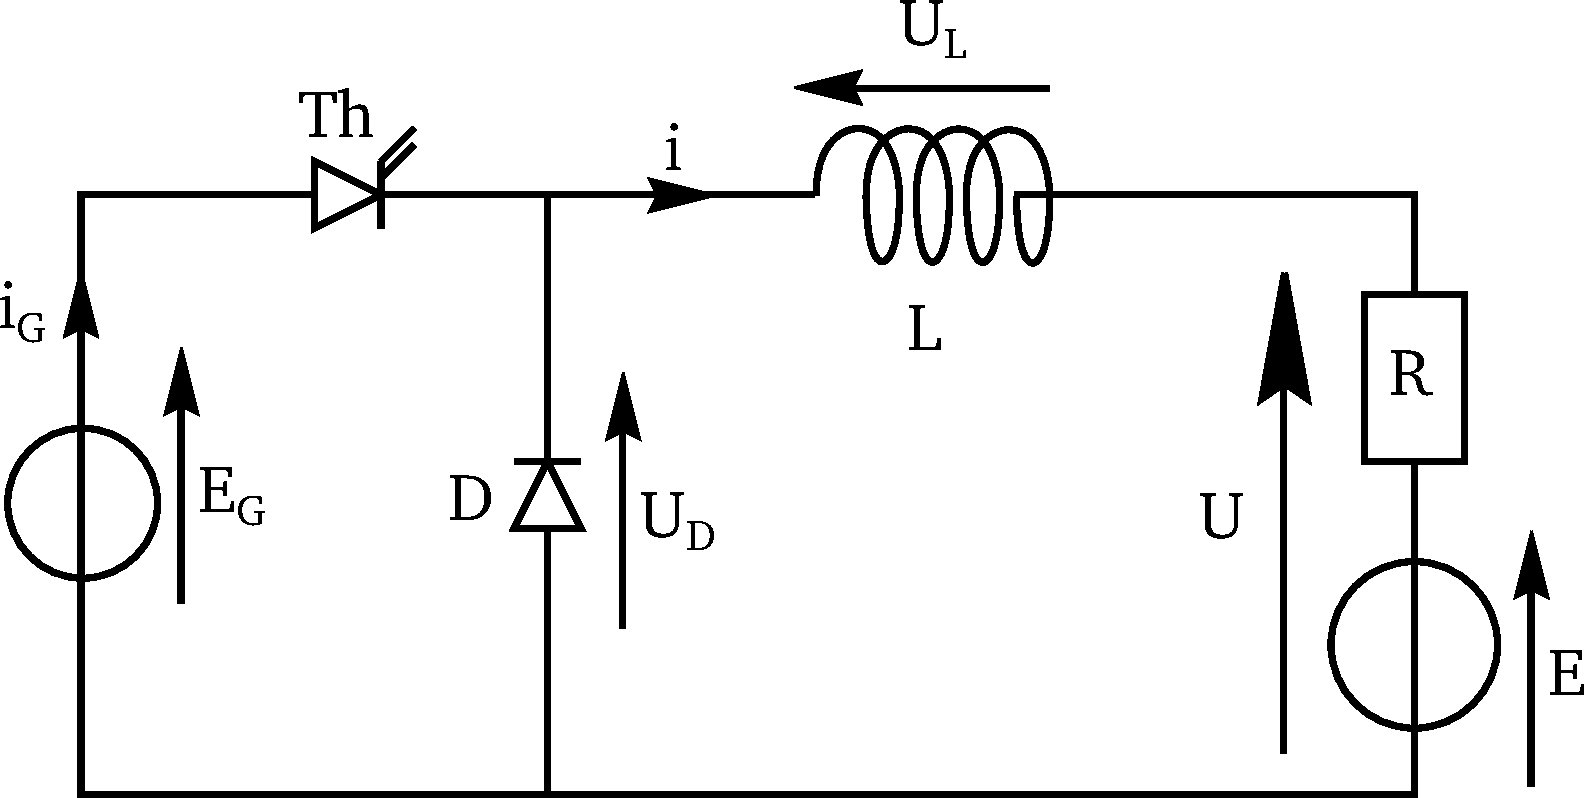
\includegraphics[scale=0.4]{Hacheur_serie.pdf}
\end{figure}	

\begin{itemize}
	\item[$\clubsuit$] Pour réaliser la condition $i$ pratiquement constante, faut-il augmenter ou diminuer l'inductance $L$ ou la période $T$ ?
	\item[$\clubsuit$] Etudier l'évolution de l'état de la diode au cours d'une période et tracer le chronogramme de $u_{D}(t)$. Quel est le signe de $i$ ?
	\item[$\clubsuit$] En régime périodique établi, déterminer les valeurs moyennes de $u_{D}(t)$, $u_{L}(t)$, $u(t)$ et $i(t)$, notées respectivement $U_{D}$, $U_{L}$, $U$ et $I$.
	\item[$\clubsuit$] En supposant $i$ constant, tracer le chronogramme de $i_{G}$, le courant débité par le générateur. Quelle est avec cette approximation sa valeur moyenne $I_{G}$ ?
	\item[$\clubsuit$] Ecrire l'équation différentielle vérifiée par $i(t)$ pendant une phase d'ouverture de $Th$. En déduire une condition pour que le taux d'ondulation $\frac{I_{max}-I_{min}}{I}$ soit inférieur à $1\%$.
\end{itemize}

\newpage

\section*{Redresseur shunt}

Partant de la tension sinusoïdale du réseau, on cherche à obtenir une tension continue présentant une ondulation la plus faible possible, par un exemple pour recharger une batterie. On considère pour l'instant le redresseur double-alternance représenté sur la figure ci-dessous, constitué d'un transformateur supposé parfait et d'un pont de Graetz, la charge étant modélisée par une résistance $R_L=1,0$ k$\Omega$. 

\begin{figure}[h!]
	\centering
		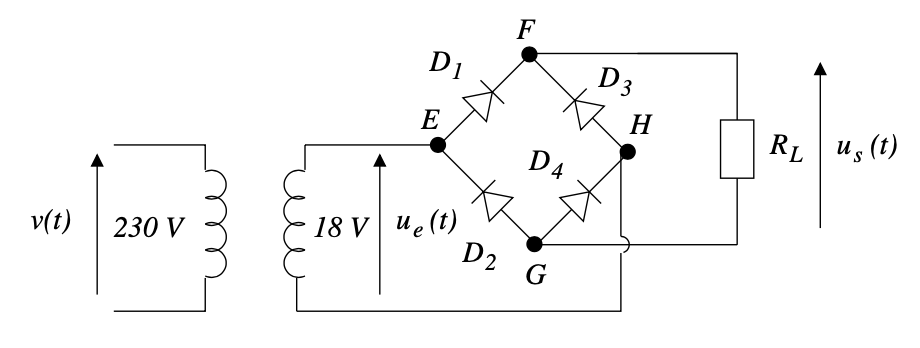
\includegraphics[scale=0.7]{circuit2_1.png}
\end{figure}	

La tension du réseau est une tension sinusoïdale de valeur efficace 230 V et de fréquence $f=1/T=50$ Hz. Le transformateur parfait convertit la tension du réseau en une tension sinusoïdale de même fréquence mais à une tension efficace de 18 V.

\begin{itemize}

	\item[$\blacksquare$] En supposant les diodes idéales, tracer la forme de la tension $u_s$ sur deux périodes du signal d'entrée. Déterminer l'amplitude, la valeur efficace et la valeur moyenne du signal de sortie $u_s$. On notera $U_e$ l'amplitude de $u_e$.
	
	\item[$\blacksquare$] Quelle est la caractéristique d'une diode réelle ? On remarque qu'en réalité, l'amplitude $U_s$ aux bornes de la résistance est de 24 V. Evaluer la tension de seuil des diodes, en supposant qu'elles sont toutes identiques. 

\end{itemize}

Afin de filtrer le signal et ne conserver que sa composante continue, on ajoute un condensateur en sortie de montage.

\begin{figure}[h!]
	\centering
		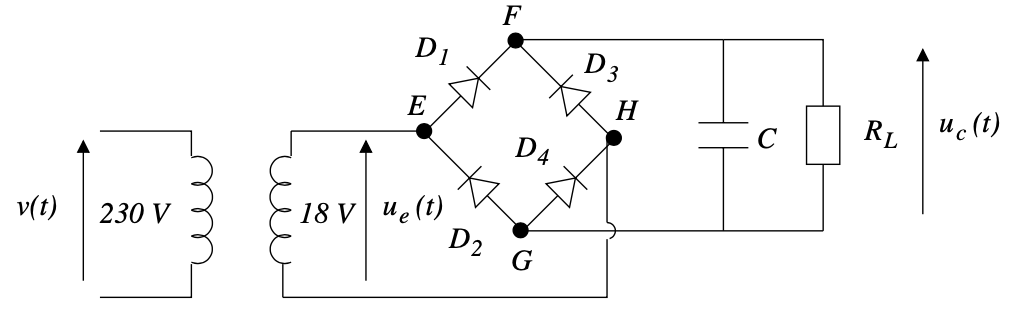
\includegraphics[scale=0.7]{circuit2_2.png}
\end{figure}	

\begin{itemize}

	\item[$\blacksquare$] En utilisant un condensateur de capacité $C=100$ $\mu$F, quelle est la durée caractéristique $\tau$ de décharge du condensateur ? Tracer l'allure de la courbe de $u_c(t)$ et justifier que l'on obtient une tension "presque" continue.

%\begin{figure}[h!]
%	\centering
%		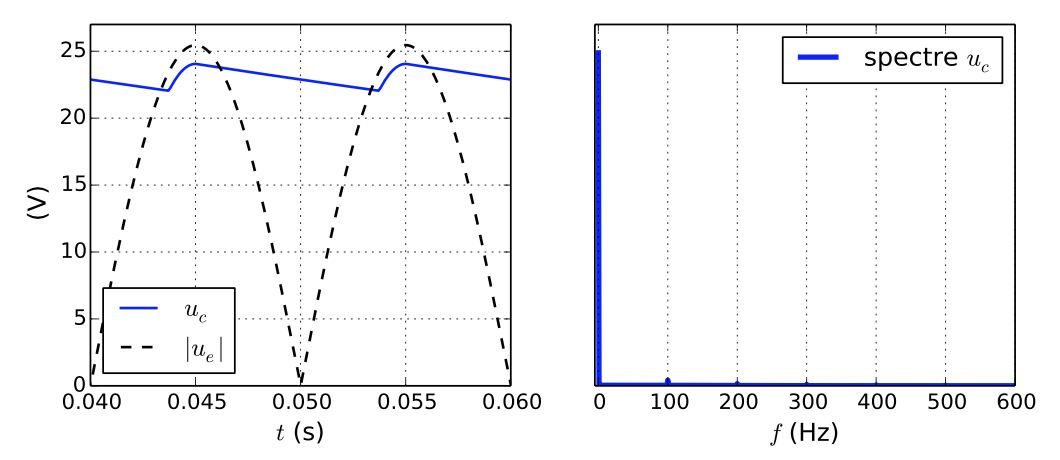
\includegraphics[scale=0.7]{courbe1.png}
%\end{figure}	

	\item[$\blacksquare$] En supposant que la décharge a lieu pendant la quasi totalité de la demi-période et que $\tau\gg T/2$, montrer que l'ondulation de tension vaut : 
	\begin{align*}
		\frac{|\Delta u_c|}{u_c^{max}}\simeq \frac{T}{2R_LC}
	\end{align*}

\end{itemize}

\end{document}